\chapter{Criptografía pública}
En este capítulo vamos  a introducir la criptografía pública.

El algoritmo en el que nos vamos a centrar en esta sección es el RSA , que es un algoritmo muy \textbf{seguro} pero muy \textbf{costoso}.

Por estas dos características el RSA no se utiliza para encriptar mensajes eteros, ya que sería un mecanismo muy lento, pero es muy útil para el intercambio de claves de la criptografía simétrica.

La robusted de la criptografía pública es similar a la factorización de números primos, que es muy costosa para números grandes.
\section{Esquema genérico de cifrado público}
\begin{center}
	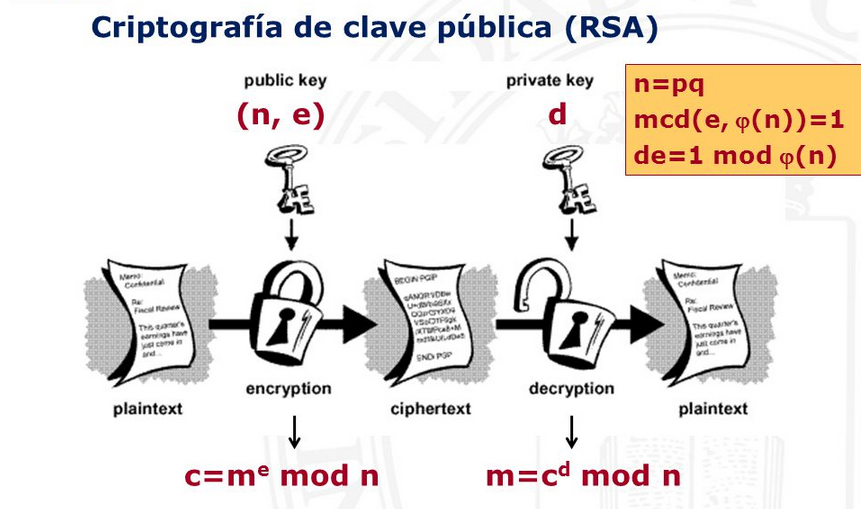
\includegraphics[width=400pt]{esquemaCpublica.png}
\end{center}



En este esquema hay una parte privada:

En la parte del Recepor tenemos el generados de claves, que genera un par de claes pública privada (e,d), de forma que la pública es la utillizada por el emisor y la privada por el receptor.

Este tipo de cifrado surge por el poblema de la distribución de claves.

La base teórica está sentada por \begin{itemize}
	\item Diffie
	\item Llellman
	\item Merkle
\end{itemize}

Y fue llevado a la práctica por primera vez por: (RSA)
\begin{itemize}
	\item Rivest
	\item Shamir
	\item Adleman
\end{itemize}

\section{Fundamentos genéricos de los cifrados asimétricos}

\begin{defn}[Funciones de una sola dirección(One Way Function)]
	\begin{enumerate}
		\item Es una función inyectiva $\rightarrow$  F: P $\rightarrow$C
		\item Cálculo de $F(x); x\in P$ es rápido
		\item Cálculo de $F(y)^{-1} ; y\in C$ es computacionalmente imposible.
	\end{enumerate}
\end{defn}

\begin{defn}[Trapdoor Function]
	\begin{enumerate}
		\item Es una función OWF (One Way Function)
		\item Dado un certificado (algún tipo de dato) , cer, entonces: $$F^{-1}_{cer}(y) ; y \in C$$
		Es computacionalmente posible
	\end{enumerate}
\end{defn}



\subsection{Funciones de una sola dirección}
¿Cómo pueden existir este tipo de funciones? Se consiguen a través de la aritmética modular.

\textbf{La aritmética modular proporciona OWF}

Vamos a poner un ejemplo para entender porqué.

\begin{example}
	
	Tenemos 
	$$x \rightarrow 1, 2, 3, 4, 5, 6, ....$$
	y la función
	$$f(x) = 3^x \rightarrow 39 , 27, 81 , 243, 729, ....$$
	
	En este caso podemos calcular la solución probando.
	
	Pero ¿si ponemos..
	$$f(x)  = 453^x \text{ mod }21997$$
	$$f(x) = 5787$$
	En este caso hay varias soluciones y no hay forma de averiguar cuál es la correcta. 
\end{example}
\subsection{Funciones Trapdoor}
\subsection{Ejemplos con aritmética modular}
\section{El algoritmo del RSA}

\subsection{Fundamentos matemáticos}
\subsection{ Generación de claves}
\begin{enumerate}
	\item Generamos 2 numeros primos p y q que cumplan:
	\begin{itemize}
		\item $p\neq q$
		\item $l_b(p)\sim l_b(q)$
	\end{itemize}
	\item Se genera $n = p\cdot q$
	$$\varphi(n) = (p-1)\cdot(q-1)$$
\end{enumerate}
\subsection{Función de cifrado RSA}
\subsection{Algoritmo de potenciación modular óptima}
\subsection{Generación de números primos grandes}
\subsection{Algoritmo de Miller-Rabin}

\subsubsection{Consideraciones Prácticas de M-R}
\begin{enumerate}
	\item Generar un N grande (n bits) aleatorio.
	\item Escribir N en binario.
	\item Dividimos N por una tabla de primos precalculados (los 2000 primeros) $\rightarrow$ el 99.8\% de los números impares es divisible entre los 2000 primeros primos.
	\item Ejecutar M-R, no una sola vez sino con muchas bases (a).
	\item Si es compuesto vuelvo a paso 2.
	
\end{enumerate}

\begin{example}
	Vamos a probar la primalidad con $p=13$
	
	Escribimos $p-1 = 12 = 2^2\cdot3$
	
	Probamos con $a = 4$
	
	Aplicando M-R vemos que 
	$$4^3 \textbf{ mod } 13 = 12$$
	$$12 = -1 \textbf{ mod } 13$$
	Con esto el test nos dice que es un posible primo
	
	Probamos con $a = 2$
	 $$2^3 \textbf{ mod } 13 = 8$$
	 $$2^{2 \cdot 3} \textbf{ mod } 13 = 12$$
	Sigue siendo un posible primo.
\end{example}

\begin{example}
	Vamos a probar la primalidad con $p = 221 = 13 \cdot 17$
	
	$n-1 = 220 = 2^2 \cdot 55$
	
	Con $a = 5$
	
	$$5^{55} \textbf{ mod } 221 = 112$$
	$$5^{2 \cdot 55} \textbf{ mod } 221 = 168$$
	
	Por lo tanto es compuesto 100\%
	
	Pero vemos que si cambiamos de base y cogemos $a=21$
	
	$$21^{55} \textbf{ mod } 221 = 200$$
	$$5^{2 \cdot 55} \textbf{ mod } 221 = 280 = -1 \textbf{ mod } 221$$
	
	Según esto sería un posible primo.
	
	Vemos que en este caso el algoritmo se equivoca.
\end{example}

\subsubsection{Equivocación de M-R}

A: Es un número impar de tamaño fijo y es compuesto

B: El algoritmo de M-R responde m veces que podría ser primo

Queremos calcular $P(B|A)$

No vamos a ver cómo se llega a esta solución pero nos dan como dato que
$$P(B|A) \leq \frac{1}{4}^m$$

\textbf{OJO! ESTA NO ES LA PROBABILIDAD DE EQUIVOCACIÓN DE M-R}

\begin{defn}[Probabilidad de error de M-R]
	Siendo A y B los casos definidos ateriormente, la probabilidad de error es:$$P(A|B)$$
	Dicha probabilidad la podemos estimar con Bayes.
\end{defn}

Vamos a ver cómo aplicaríamos Bayes:
$$P(A|B) = \frac{P(B|A)P(A)}{P(B)}$$
$$P(B) = P(B|A)P(A) + P(B|\overline{A})P(\overline{A})$$
Siendo $\overline{A}$ el caso en el que A es primo y $A$ el caso en el que A es compuesto.
$$P(A|B) = \frac{P(B|A)P(A)}{P(B|A)P(A) + P(B|\overline{A})P(\overline{A})}$$

Vemos que $P(B|\overline{A}) = 1$

¿Cómo calculamos $P(\overline{A})$?¿Cuál es la probabilidad de tener números prims de tamaño fijo(n bits)?

Conjetura de Gauss

El número de primos del intervalo {0-N} es $\approx \frac{N}{\log N}$

$$\lim_{N\rightarrow \infty} \frac{\Pi(N)}{\frac{N}{\log N}} \rightarrow 1$$

Como N tiene n bits $\implies N = 2^n$

Por la conjetura de Gauss la probabilidad entonces en el intervalo ${0, 2^n}$ es
$$\frac{2^n}{\log 2^n}$$

Y ahora el número de primos de n bits es:
$$\frac{2^n}{\log 2^n} - \frac{2^{n-1}}{\log 2^{n-1}} = \frac{2^n}{n \cdot\log 2}- \frac{2^n}{(n-1)\cdot\log 2} =$$
$$ = \frac{2^{n-1}}{log 2}(\frac{2}{n} - \frac{1}{n-1}) = \frac{2^{n-1}}{n \cdot log2}$$

Con esto ya podemos clacular $P(\overline{A})$
$$P(\overline{A}) = \frac{\frac{2^{n-1}}{n \cdot log2}}{2^{n-1}} \approx\frac{1}{n \cdot log 2}$$

Finalmente tenemos que:
$$P(A|B) = \frac{(1/n)^m (1- \frac{1}{n \cdot log 2})}{(1/n)^m (1 - \frac{1}{n \cdot log 2}) + \frac{1}{n \cdot log 2}} = \frac{(1/n)^m (n \cdot log 2 -1)}{(1/n)^m (n \cdot log 2 -1) +1} = ... \approx\frac{1}{1+ \frac{4^m}{n\cdot log 2}}$$

Ahora vamos a ver cómo podemos utilizar esta probabilidad.


\begin{center}
	
	\begin{tabular}{l | c  r}
		$P(A|B)$ & m & n \\
		\hline
	0.0107 & 8 & 1024 \\
	\hline
		$1.6526 \cdot 10^{-7}$ & 16 & 1024\\
		\hline
	$8.2630 \cdot 10^{-8}$ & 16 & 512 \\
		\hline
		$8.8477 \cdot 10^{-17}$ & 32 & 1024
	
	\end{tabular}
\end{center}



\subsection{Primos fuertes}
\subsection{Inyectividad del RSA}
\subsection{Tipos de ataques y vulnerabilidades sobre el RSA}